
%% bare_conf.tex
%% V1.3
%% 2007/01/11
%% by Michael Shell
%% See:
%% http://www.michaelshell.org/
%% for current contact information.
%%
%% This is a skeleton file demonstrating the use of IEEEtran.cls
%% (requires IEEEtran.cls version 1.7 or later) with an IEEE conference paper.
%%
%% Support sites:
%% http://www.michaelshell.org/tex/ieeetran/
%% http://www.ctan.org/tex-archive/macros/latex/contrib/IEEEtran/
%% and
%% http://www.ieee.org/

%%*************************************************************************
%% Legal Notice:
%% This code is offered as-is without any warranty either expressed or
%% implied; without even the implied warranty of MERCHANTABILITY or
%% FITNESS FOR A PARTICULAR PURPOSE! 
%% User assumes all risk.
%% In no event shall IEEE or any contributor to this code be liable for
%% any damages or losses, including, but not limited to, incidental,
%% consequential, or any other damages, resulting from the use or misuse
%% of any information contained here.
%%
%% All comments are the opinions of their respective authors and are not
%% necessarily endorsed by the IEEE.
%%
%% This work is distributed under the LaTeX Project Public License (LPPL)
%% ( http://www.latex-project.org/ ) version 1.3, and may be freely used,
%% distributed and modified. A copy of the LPPL, version 1.3, is included
%% in the base LaTeX documentation of all distributions of LaTeX released
%% 2003/12/01 or later.
%% Retain all contribution notices and credits.
%% ** Modified files should be clearly indicated as such, including  **
%% ** renaming them and changing author support contact information. **
%%
%% File list of work: IEEEtran.cls, IEEEtran_HOWTO.pdf, bare_adv.tex,
%%                    bare_conf.tex, bare_jrnl.tex, bare_jrnl_compsoc.tex
%%*************************************************************************

% *** Authors should verify (and, if needed, correct) their LaTeX system  ***
% *** with the testflow diagnostic prior to trusting their LaTeX platform ***
% *** with production work. IEEE's font choices can trigger bugs that do  ***
% *** not appear when using other class files.                            ***
% The testflow support page is at:
% http://www.michaelshell.org/tex/testflow/



% Note that the a4paper option is mainly intended so that authors in
% countries using A4 can easily print to A4 and see how their papers will
% look in print - the typesetting of the document will not typically be
% affected with changes in paper size (but the bottom and side margins will).
% Use the testflow package mentioned above to verify correct handling of
% both paper sizes by the user's LaTeX system.
%
% Also note that the "draftcls" or "draftclsnofoot", not "draft", option
% should be used if it is desired that the figures are to be displayed in
% draft mode.
%
\documentclass[conference]{IEEEtran}
% Add the compsoc option for Computer Society conferences.
%
% If IEEEtran.cls has not been installed into the LaTeX system files,
% manually specify the path to it like:
% \documentclass[conference]{../sty/IEEEtran}


\usepackage{subfigure}
\usepackage{graphicx} 
\usepackage{listings}
\usepackage{color}

\definecolor{dunkelgrau}{rgb}{0.8,0.8,0.8}
% \renewcommand{\chaptername}{}
% \renewcommand{\thechapter}{}

\lstdefinestyle{customc}{
  belowcaptionskip=1\baselineskip,
  breaklines=true,
  frame=L,
  xleftmargin=\parindent,
  language=C,
  showstringspaces=false,
  basicstyle=\footnotesize\ttfamily,
%  keywordstyle=\bfseries\color{green},
  commentstyle=\itshape\color{green},
%   identifierstyle=\color{blue},
  stringstyle=\color{red},  
% 	      basicstyle=\footnotesize,% basic font setting
 	      frame=single,
% 	      commentstyle=\color{green},
 	      escapeinside={\%*}{*)},
% 	      keepspaces=true,
 	      keywordstyle=\color{blue},
 	      numbers=left,
 	      numbersep=5pt,
 	      numberstyle=\tiny\color{dunkelgrau},
 	      rulecolor=\color{black}, 
 	      stepnumber=1,
% 	      stringstyle=\color{mauve},
 	      tabsize=2, 
}

\lstset{escapechar=@,style=customc}

% Some very useful LaTeX packages include:
% (uncomment the ones you want to load)


% *** MISC UTILITY PACKAGES ***
%
%\usepackage{ifpdf}
% Heiko Oberdiek's ifpdf.sty is very useful if you need conditional
% compilation based on whether the output is pdf or dvi.
% usage:
% \ifpdf
%   % pdf code
% \else
%   % dvi code
% \fi
% The latest version of ifpdf.sty can be obtained from:
% http://www.ctan.org/tex-archive/macros/latex/contrib/oberdiek/
% Also, note that IEEEtran.cls V1.7 and later provides a builtin
% \ifCLASSINFOpdf conditional that works the same way.
% When switching from latex to pdflatex and vice-versa, the compiler may
% have to be run twice to clear warning/error messages.






% *** CITATION PACKAGES ***
%
%\usepackage{cite}
% cite.sty was written by Donald Arseneau
% V1.6 and later of IEEEtran pre-defines the format of the cite.sty package
% \cite{} output to follow that of IEEE. Loading the cite package will
% result in citation numbers being automatically sorted and properly
% "compressed/ranged". e.g., [1], [9], [2], [7], [5], [6] without using
% cite.sty will become [1], [2], [5]--[7], [9] using cite.sty. cite.sty's
% \cite will automatically add leading space, if needed. Use cite.sty's
% noadjust option (cite.sty V3.8 and later) if you want to turn this off.
% cite.sty is already installed on most LaTeX systems. Be sure and use
% version 4.0 (2003-05-27) and later if using hyperref.sty. cite.sty does
% not currently provide for hyperlinked citations.
% The latest version can be obtained at:
% http://www.ctan.org/tex-archive/macros/latex/contrib/cite/
% The documentation is contained in the cite.sty file itself.






% *** GRAPHICS RELATED PACKAGES ***
%
\ifCLASSINFOpdf
  % \usepackage[pdftex]{graphicx}
  % declare the path(s) where your graphic files are
  % \graphicspath{{../pdf/}{../jpeg/}}
  % and their extensions so you won't have to specify these with
  % every instance of \includegraphics
  % \DeclareGraphicsExtensions{.pdf,.jpeg,.png}
\else
  % or other class option (dvipsone, dvipdf, if not using dvips). graphicx
  % will default to the driver specified in the system graphics.cfg if no
  % driver is specified.
  % \usepackage[dvips]{graphicx}
  % declare the path(s) where your graphic files are
  % \graphicspath{{../eps/}}
  % and their extensions so you won't have to specify these with
  % every instance of \includegraphics
  % \DeclareGraphicsExtensions{.eps}
\fi
% graphicx was written by David Carlisle and Sebastian Rahtz. It is
% required if you want graphics, photos, etc. graphicx.sty is already
% installed on most LaTeX systems. The latest version and documentation can
% be obtained at: 
% http://www.ctan.org/tex-archive/macros/latex/required/graphics/
% Another good source of documentation is "Using Imported Graphics in
% LaTeX2e" by Keith Reckdahl which can be found as epslatex.ps or
% epslatex.pdf at: http://www.ctan.org/tex-archive/info/
%
% latex, and pdflatex in dvi mode, support graphics in encapsulated
% postscript (.eps) format. pdflatex in pdf mode supports graphics
% in .pdf, .jpeg, .png and .mps (metapost) formats. Users should ensure
% that all non-photo figures use a vector format (.eps, .pdf, .mps) and
% not a bitmapped formats (.jpeg, .png). IEEE frowns on bitmapped formats
% which can result in "jaggedy"/blurry rendering of lines and letters as
% well as large increases in file sizes.
%
% You can find documentation about the pdfTeX application at:
% http://www.tug.org/applications/pdftex





% *** MATH PACKAGES ***
%
%\usepackage[cmex10]{amsmath}
% A popular package from the American Mathematical Society that provides
% many useful and powerful commands for dealing with mathematics. If using
% it, be sure to load this package with the cmex10 option to ensure that
% only type 1 fonts will utilized at all point sizes. Without this option,
% it is possible that some math symbols, particularly those within
% footnotes, will be rendered in bitmap form which will result in a
% document that can not be IEEE Xplore compliant!
%
% Also, note that the amsmath package sets \interdisplaylinepenalty to 10000
% thus preventing page breaks from occurring within multiline equations. Use:
%\interdisplaylinepenalty=2500
% after loading amsmath to restore such page breaks as IEEEtran.cls normally
% does. amsmath.sty is already installed on most LaTeX systems. The latest
% version and documentation can be obtained at:
% http://www.ctan.org/tex-archive/macros/latex/required/amslatex/math/





% *** SPECIALIZED LIST PACKAGES ***
%
%\usepackage{algorithmic}
% algorithmic.sty was written by Peter Williams and Rogerio Brito.
% This package provides an algorithmic environment fo describing algorithms.
% You can use the algorithmic environment in-text or within a figure
% environment to provide for a floating algorithm. Do NOT use the algorithm
% floating environment provided by algorithm.sty (by the same authors) or
% algorithm2e.sty (by Christophe Fiorio) as IEEE does not use dedicated
% algorithm float types and packages that provide these will not provide
% correct IEEE style captions. The latest version and documentation of
% algorithmic.sty can be obtained at:
% http://www.ctan.org/tex-archive/macros/latex/contrib/algorithms/
% There is also a support site at:
% http://algorithms.berlios.de/index.html
% Also of interest may be the (relatively newer and more customizable)
% algorithmicx.sty package by Szasz Janos:
% http://www.ctan.org/tex-archive/macros/latex/contrib/algorithmicx/




% *** ALIGNMENT PACKAGES ***
%
%\usepackage{array}
% Frank Mittelbach's and David Carlisle's array.sty patches and improves
% the standard LaTeX2e array and tabular environments to provide better
% appearance and additional user controls. As the default LaTeX2e table
% generation code is lacking to the point of almost being broken with
% respect to the quality of the end results, all users are strongly
% advised to use an enhanced (at the very least that provided by array.sty)
% set of table tools. array.sty is already installed on most systems. The
% latest version and documentation can be obtained at:
% http://www.ctan.org/tex-archive/macros/latex/required/tools/


%\usepackage{mdwmath}
%\usepackage{mdwtab}
% Also highly recommended is Mark Wooding's extremely powerful MDW tools,
% especially mdwmath.sty and mdwtab.sty which are used to format equations
% and tables, respectively. The MDWtools set is already installed on most
% LaTeX systems. The lastest version and documentation is available at:
% http://www.ctan.org/tex-archive/macros/latex/contrib/mdwtools/


% IEEEtran contains the IEEEeqnarray family of commands that can be used to
% generate multiline equations as well as matrices, tables, etc., of high
% quality.


%\usepackage{eqparbox}
% Also of notable interest is Scott Pakin's eqparbox package for creating
% (automatically sized) equal width boxes - aka "natural width parboxes".
% Available at:
% http://www.ctan.org/tex-archive/macros/latex/contrib/eqparbox/





% *** SUBFIGURE PACKAGES ***
%\usepackage[tight,footnotesize]{subfigure}
% subfigure.sty was written by Steven Douglas Cochran. This package makes it
% easy to put subfigures in your figures. e.g., "Figure 1a and 1b". For IEEE
% work, it is a good idea to load it with the tight package option to reduce
% the amount of white space around the subfigures. subfigure.sty is already
% installed on most LaTeX systems. The latest version and documentation can
% be obtained at:
% http://www.ctan.org/tex-archive/obsolete/macros/latex/contrib/subfigure/
% subfigure.sty has been superceeded by subfig.sty.



%\usepackage[caption=false]{caption}
%\usepackage[font=footnotesize]{subfig}
% subfig.sty, also written by Steven Douglas Cochran, is the modern
% replacement for subfigure.sty. However, subfig.sty requires and
% automatically loads Axel Sommerfeldt's caption.sty which will override
% IEEEtran.cls handling of captions and this will result in nonIEEE style
% figure/table captions. To prevent this problem, be sure and preload
% caption.sty with its "caption=false" package option. This is will preserve
% IEEEtran.cls handing of captions. Version 1.3 (2005/06/28) and later 
% (recommended due to many improvements over 1.2) of subfig.sty supports
% the caption=false option directly:
%\usepackage[caption=false,font=footnotesize]{subfig}
%
% The latest version and documentation can be obtained at:
% http://www.ctan.org/tex-archive/macros/latex/contrib/subfig/
% The latest version and documentation of caption.sty can be obtained at:
% http://www.ctan.org/tex-archive/macros/latex/contrib/caption/




% *** FLOAT PACKAGES ***
%
%\usepackage{fixltx2e}
% fixltx2e, the successor to the earlier fix2col.sty, was written by
% Frank Mittelbach and David Carlisle. This package corrects a few problems
% in the LaTeX2e kernel, the most notable of which is that in current
% LaTeX2e releases, the ordering of single and double column floats is not
% guaranteed to be preserved. Thus, an unpatched LaTeX2e can allow a
% single column figure to be placed prior to an earlier double column
% figure. The latest version and documentation can be found at:
% http://www.ctan.org/tex-archive/macros/latex/base/



%\usepackage{stfloats}
% stfloats.sty was written by Sigitas Tolusis. This package gives LaTeX2e
% the ability to do double column floats at the bottom of the page as well
% as the top. (e.g., "\begin{figure*}[!b]" is not normally possible in
% LaTeX2e). It also provides a command:
%\fnbelowfloat
% to enable the placement of footnotes below bottom floats (the standard
% LaTeX2e kernel puts them above bottom floats). This is an invasive package
% which rewrites many portions of the LaTeX2e float routines. It may not work
% with other packages that modify the LaTeX2e float routines. The latest
% version and documentation can be obtained at:
% http://www.ctan.org/tex-archive/macros/latex/contrib/sttools/
% Documentation is contained in the stfloats.sty comments as well as in the
% presfull.pdf file. Do not use the stfloats baselinefloat ability as IEEE
% does not allow \baselineskip to stretch. Authors submitting work to the
% IEEE should note that IEEE rarely uses double column equations and
% that authors should try to avoid such use. Do not be tempted to use the
% cuted.sty or midfloat.sty packages (also by Sigitas Tolusis) as IEEE does
% not format its papers in such ways.





% *** PDF, URL AND HYPERLINK PACKAGES ***
%
%\usepackage{url}
% url.sty was written by Donald Arseneau. It provides better support for
% handling and breaking URLs. url.sty is already installed on most LaTeX
% systems. The latest version can be obtained at:
% http://www.ctan.org/tex-archive/macros/latex/contrib/misc/
% Read the url.sty source comments for usage information. Basically,
% \url{my_url_here}.





% *** Do not adjust lengths that control margins, column widths, etc. ***
% *** Do not use packages that alter fonts (such as pslatex).         ***
% There should be no need to do such things with IEEEtran.cls V1.6 and later.
% (Unless specifically asked to do so by the journal or conference you plan
% to submit to, of course. )


% correct bad hyphenation here
\hyphenation{op-tical net-works semi-conduc-tor}


\begin{document}
%
% paper title
% can use linebreaks \\ within to get better formatting as desired
\title{IS2200 - Parallel Computer Systems \\{Lab1: Maximum sub-array problem}}


% author names and affiliations
% use a multiple column layout for up to three different
% affiliations
\author{\IEEEauthorblockN{Elias Marquart}
\IEEEauthorblockA{School of Computer Science and Communication\\
Royal Institute of Technology, Stockholm\\
Email: FIXME.se}
\and
\IEEEauthorblockN{Sergej Proskurin}
\IEEEauthorblockA{School of Information and Communication Technology\\
Royal Institute of Technology, Stockholm\\
Email: sergejp@kth.se}}


% conference papers do not typically use \thanks and this command
% is locked out in conference mode. If really needed, such as for
% the acknowledgment of grants, issue a \IEEEoverridecommandlockouts
% after \documentclass

% for over three affiliations, or if they all won't fit within the width
% of the page, use this alternative format:
% 
%\author{\IEEEauthorblockN{Michael Shell\IEEEauthorrefmark{1},
%Homer Simpson\IEEEauthorrefmark{2},
%James Kirk\IEEEauthorrefmark{3}, 
%Montgomery Scott\IEEEauthorrefmark{3} and
%Eldon Tyrell\IEEEauthorrefmark{4}}
%\IEEEauthorblockA{\IEEEauthorrefmark{1}School of Electrical and Computer Engineering\\
%Georgia Institute of Technology,
%Atlanta, Georgia 30332--0250\\ Email: see http://www.michaelshell.org/contact.html}
%\IEEEauthorblockA{\IEEEauthorrefmark{2}Twentieth Century Fox, Springfield, USA\\
%Email: homer@thesimpsons.com}
%\IEEEauthorblockA{\IEEEauthorrefmark{3}Starfleet Academy, San Francisco, California 96678-2391\\
%Telephone: (800) 555--1212, Fax: (888) 555--1212}
%\IEEEauthorblockA{\IEEEauthorrefmark{4}Tyrell Inc., 123 Replicant Street, Los Angeles, California 90210--4321}}




% use for special paper notices
%\IEEEspecialpapernotice{(Invited Paper)}




% make the title area
\maketitle


\begin{abstract}
%\boldmath
The abstract goes here.
\end{abstract}
% IEEEtran.cls defaults to using nonbold math in the Abstract.
% This preserves the distinction between vectors and scalars. However,
% if the conference you are submitting to favors bold math in the abstract,
% then you can use LaTeX's standard command \boldmath at the very start
% of the abstract to achieve this. Many IEEE journals/conferences frown on
% math in the abstract anyway.

% no keywords




% For peer review papers, you can put extra information on the cover
% page as needed:
% \ifCLASSOPTIONpeerreview
% \begin{center} \bfseries EDICS Category: 3-BBND \end{center}
% \fi
%
% For peerreview papers, this IEEEtran command inserts a page break and
% creates the second title. It will be ignored for other modes.
\IEEEpeerreviewmaketitle



\section{Introduction}
% no \IEEEPARstart
In the context of the labwork of the course Parallel Computer Systems, a reference of the maximum sum-array problem implementation had to be extended in such a way that it would be able to scale on a large number of cores. In this paper, we discuss two solutions, where one of the solutions implements an explicit threading model with help of POSIX threads and the second solution makes use of the programming framework OpenMP and hence implementing an implicit threading model. 

Section \ref{sec:impl} shortly introduces the initial modifications of the given reference implementation of the maximum sub-array problem and further discusses the implementation of both solutions using explicit threading and implicit threading techniques and their associated parallel patterns. Subsequently, section \ref{sec:analysis} presents performance analysis - in terms of speedup and efficiency - of the maximum sub-array problem using both imlementation solutions on different architectures. Finally, to conclude this paper, section \ref{sec:conclusion} rounds up the discussion by providing a short comparison between the used implementation techniques. 

\section{Implementation}
\label{sec:impl}

Before we begin the discussion about the used implementation techniques (section \ref{sec:impl:pthread} and \ref{sec:impl:openmp}), we would like to present modifications of the initial reference implementation of the maximum sub-array problem (section \ref{sec:impl:modifications}). 

\subsection{Initial Program Modifications}
\label{sec:impl:modifications}

After studying the initial reference implementation, we decomposed this implementation into multiple functions, which we could better analyse using profilers, such as valgrind\cite{VALGRIND}. In total, three different code optimizations have been performed before parallelization techniques were applied to the initial implementation.  

First, after analysing the profiler results, it turned out that the function \texttt{clear()} is used very often in comparison to the most of the other functions within the implementation. According to valgrind (figure \ref{pic:clear}), in the initial implementation \texttt{clear()} is called over 250.000 times with an input matrix dimension of 500x500. Thus, it requires about 22.31\% of the total execution time to perform the \texttt{clear()} operations (figure \ref{pic:clear} a).  

\begin{figure}[h]
  \centering
  \subfigure[Unoptimized]{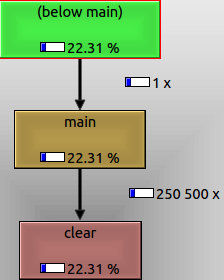
\includegraphics[scale=0.42]{pic/clear.png}}\quad
  \subfigure[Optimized]{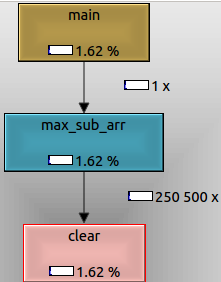
\includegraphics[scale=0.42]{pic/clear2.png}}
  \caption{Profiling Clear Function}
  \label{pic:clear}
\end{figure}

It turned out that a simple \texttt{memset()} function was able to reduce the runtime of the \texttt{clear()} function to only 1.62\% of the total execution time of the program (figure \ref{pic:clear} b).

A similar performance improvement could be done for the output matrix initialization (listing \ref{lst:outmat}), respectively, by simply using the function \texttt{memcpy()} (listing \ref{lst:outmat-opt}). Thus, it was possible to make the code shown in listing \ref{lst:outmat} faster. But since this part of the code was executed only once, it did not contribute significantly to the total execution time. 

\begin{center}
   \begin{lstlisting}[captionpos=b, caption=Initial Implementation: Initialize Output Matrix, label=lst:outmat]
for(int i=top, k=0; i<=bottom; i++,k++) {     
    for(int j=left,l=0; j<=right; j++,l++) {
        outmat[k][l] = mat[i][j];              
    }                                          
}                                              
   \end{lstlisting}
\end{center}

\begin{center}
   \begin{lstlisting}[captionpos=b, caption=Optimized Implementation: Initialize Output Matrix, label=lst:outmat-opt]  
for(int i=top, k=0; i<=bottom; i++, k++) {                                       
    int j=left;                                                                                    
    memcpy((void*)outmat[k],(void*)(&mat[i][j]),
            sizeof(**mat)*(right-left+1));                                          
}                                                 
   \end{lstlisting}
\end{center}
   
The third code modification comprised heap memory allocation for the used matrices within the code. Since matrices on the stack are limited by the actual stack size, we decided to allocate enough memory on the heap with help of \texttt{malloc()}.

   
\subsection{Explicit Multi-Threading - POSIX Threads}
\label{sec:impl:pthread}



\subsection{Implicit Multi-Threading - OpenMP}
\label{sec:impl:openmp}

In order to make better use of the parallel hardware, we decided to use implicit multi-threading framework OpenMP. OpenMP is able to fork a specific number of children, which then execute independently a specified region of code. OpenMP enables in contrast to explicit multi-threading approaches an easy implementation, which simultaneously performs and scales very well. In order to parallelize the initial implementation with help of OpenMP, we had to extend the initial code on only two places without major code modification - which speaks for the ease of OpenMP. 

First, we parallelized the the matrix precomputation of the vertical prefix sum, comprised of a double for loop, by simply adding an OpenMP compiler directive (listing \ref{lst:precomp}).

\begin{center}
   \begin{lstlisting}[captionpos=b, caption=OpenMP: Parallel Matrix Pre-Computation of the Vertical Sum, label=lst:precomp]                                            
void precomp_matrix(int **mat, int **ps, int dim)                                  
{                                             
    /* precompute vertical prefix sum */  
    #pragma omp parallel for \ 
        default(none) \        
        firstprivate(dim) \    
        shared(ps, mat) \      
        if(dim > 8) \          
        schedule(static) \     
        num_threads(thread_nr)     
    for(int j=0; j<dim; j++) {                
        ps[0][j] = mat[0][j];                 
        for (int i=1; i<dim; i++) {           
            ps[i][j] = ps[i-1][j] + mat[i][j];
        }                                     
    }                                         
}                                             
   \end{lstlisting}
\end{center}

The OpenMP compiler \texttt{parallel for} directive in listing \ref{lst:precomp} parallelizes the for loop by internally forking \texttt{thread\_nr} times and organizing the individual threads in such a way that they are able to work on individual ranges of the for loop. We have implemented the if(dim>8) directive, since according do measurements, it simply does not make sence to fork if you have only a small number of values to compute; False sharing might be as well a potential issue. 

We have explicitely stated all shared and private variables in order to follow the good practice of an OpenMP implementation. In this case, the stated shared and private variables do not make significant code improvements; however, they can result in a huge runtime improvement when dealing with cache coherence issues on multicore-processors resulting in false sharing. 

The reason why we do not experience false sharing (or at least only at a small rate) is that the first for loop iterates through columns (not rows) and hence individual threads, potentially running on different cores, experience a bigger memory distance within the array \texttt{ps}. If we would parallelize the inner for loop, we would get into troubles, since the memory positions, accessed by different threads, would be too close to each other and eventually lead to false sharing. 

The second and last code extension of the initial implementation affects the main algorithm. At this point, we considered two different solutions, whereas both of them scaled very well and performed almost similar. The first solution shared the variables \texttt{max\_sum}, \texttt{top}, \texttt{bottom}, \texttt{left}, and \texttt{right}. In order to synchronize the individual threads, we used a \texttt{critical} section (in this case it is not possible to use an \texttt{atomic} statement instead), whose performance impact was lindered by the \texttt{flush} statement, since this way the threads on individual cores were able to be informed about the most recent value of \texttt{max\_sum} and often skipped the critical section. 


\begin{center}
   \begin{lstlisting}[captionpos=b, caption=OpenMP: Parallel Main Algorithm, label=lst:alg]  
void max_sub_arr(int **mat, int **ps, 
        int **outmat, int dim)                                                   
{                                                              
    ... 
    for(int i=0; i<dim; i++) {
        #pragma omp parallel for \
            default(none) \
            schedule(static) \
            firstprivate(dim, i) \
            private(sum, pos, local_max) \
            shared(max_sum, top, bottom, 
                left, right, ps)
            num_threads(thread_nr)
        for(int k=i; k<dim; k++) { 
            ...
            #pragma omp flush (max_sum)       
            if(sum[local_max] > max_sum) {    
                #pragma omp critical          
                if(sum[local_max] > max_sum) {
                    ...
                }
            }              
        }
    }
}
   \end{lstlisting}
\end{center}	

As already mentioned, this implementation scaled and performed well but in the end, we implemented another solution, without \texttt{critical} and \texttt{flush} statements and hence increased performance a little bit more. Therefore, we used a similar approach as witihin the pthread implementation in section \ref{sec:impl:pthread}. Within the parallel for loop, we used local copies of the critical variables, stored within the struct tr, whose results were processed by the single master thread after the for loop and hence established consistency. 


\begin{center}
   \begin{lstlisting}[captionpos=b, caption=OpenMP: Parallel Main Algorithm, label=lst:alg]  
void max_sub_arr(int **mat, int **ps,                                                  
        int **outmat, int dim)                                                   
{                                                              
    ...                                        
    for(int i=0; i<dim; i++) {                                 
        #pragma omp parallel for \                             
            default(none) \                                    
            schedule(static) \                                 
            firstprivate(dim, i) \                             
            private(sum, pos, local_max) \                     
            shared(ps, tr) \                                   
            num_threads(thread_nr)                                                                                          
        for(int k=i; k<dim; k++) { 
            ...
        }
    }
}
   \end{lstlisting}
\end{center}



\section{Analysis of Performance}
\label{sec:analysis}

% FIXME GCC vs ICC!!!

\subsection{Explicit Threading - POSIX Threads}
\label{sec:analysis:pthread}



\subsection{Implicit Threading - OpenMP}
\label{sec:analysis:openmp}


% An example of a floating figure using the graphicx package.
% Note that \label must occur AFTER (or within) \caption.
% For figures, \caption should occur after the \includegraphics.
% Note that IEEEtran v1.7 and later has special internal code that
% is designed to preserve the operation of \label within \caption
% even when the captionsoff option is in effect. However, because
% of issues like this, it may be the safest practice to put all your
% \label just after \caption rather than within \caption{}.
%
% Reminder: the "draftcls" or "draftclsnofoot", not "draft", class
% option should be used if it is desired that the figures are to be
% displayed while in draft mode.
%
%\begin{figure}[!t]
%\centering
%\includegraphics[width=2.5in]{myfigure}
% where an .eps filename suffix will be assumed under latex, 
% and a .pdf suffix will be assumed for pdflatex; or what has been declared
% via \DeclareGraphicsExtensions.
%\caption{Simulation Results}
%\label{fig_sim}
%\end{figure}

% Note that IEEE typically puts floats only at the top, even when this
% results in a large percentage of a column being occupied by floats.


% An example of a double column floating figure using two subfigures.
% (The subfig.sty package must be loaded for this to work.)
% The subfigure \label commands are set within each subfloat command, the
% \label for the overall figure must come after \caption.
% \hfil must be used as a separator to get equal spacing.
% The subfigure.sty package works much the same way, except \subfigure is
% used instead of \subfloat.
%
%\begin{figure*}[!t]
%\centerline{\subfloat[Case I]\includegraphics[width=2.5in]{subfigcase1}%
%\label{fig_first_case}}
%\hfil
%\subfloat[Case II]{\includegraphics[width=2.5in]{subfigcase2}%
%\label{fig_second_case}}}
%\caption{Simulation results}
%\label{fig_sim}
%\end{figure*}
%
% Note that often IEEE papers with subfigures do not employ subfigure
% captions (using the optional argument to \subfloat), but instead will
% reference/describe all of them (a), (b), etc., within the main caption.


% An example of a floating table. Note that, for IEEE style tables, the 
% \caption command should come BEFORE the table. Table text will default to
% \footnotesize as IEEE normally uses this smaller font for tables.
% The \label must come after \caption as always.
%
%\begin{table}[!t]
%% increase table row spacing, adjust to taste
%\renewcommand{\arraystretch}{1.3}
% if using array.sty, it might be a good idea to tweak the value of
% \extrarowheight as needed to properly center the text within the cells
%\caption{An Example of a Table}
%\label{table_example}
%\centering
%% Some packages, such as MDW tools, offer better commands for making tables
%% than the plain LaTeX2e tabular which is used here.
%\begin{tabular}{|c||c|}
%\hline
%One & Two\\
%\hline
%Three & Four\\
%\hline
%\end{tabular}
%\end{table}


% Note that IEEE does not put floats in the very first column - or typically
% anywhere on the first page for that matter. Also, in-text middle ("here")
% positioning is not used. Most IEEE journals/conferences use top floats
% exclusively. Note that, LaTeX2e, unlike IEEE journals/conferences, places
% footnotes above bottom floats. This can be corrected via the \fnbelowfloat
% command of the stfloats package.





\section{Conclusion}
\label{sec:conclusion}




% conference papers do not normally have an appendix


% use section* for acknowledgement
% \section*{Acknowledgment}
% 
% 
% The authors would like to thank...





% trigger a \newpage just before the given reference
% number - used to balance the columns on the last page
% adjust value as needed - may need to be readjusted if
% the document is modified later
%\IEEEtriggeratref{8}
% The "triggered" command can be changed if desired:
%\IEEEtriggercmd{\enlargethispage{-5in}}

% references section

% can use a bibliography generated by BibTeX as a .bbl file
% BibTeX documentation can be easily obtained at:
% http://www.ctan.org/tex-archive/biblio/bibtex/contrib/doc/
% The IEEEtran BibTeX style support page is at:
% http://www.michaelshell.org/tex/ieeetran/bibtex/
%\bibliographystyle{IEEEtran}
% argument is your BibTeX string definitions and bibliography database(s)
%\bibliography{IEEEabrv,../bib/paper}
%
% <OR> manually copy in the resultant .bbl file
% set second argument of \begin to the number of references
% (used to reserve space for the reference number labels box)


\begin{thebibliography}{1}
% 
\bibitem{VALGRIND}
(2013, Nov.) The Valgrind website. [Online]. Available: http://www.valgrind.org/
% H.~Kopka and P.~W. Daly, \emph{A Guide to \LaTeX}, 3rd~ed.\hskip 1em plus
%   0.5em minus 0.4em\relax Harlow, England: Addison-Wesley, 1999.
% 
\end{thebibliography}




% that's all folks
\end{document}


